\begin{mydef}
	Une \kw{\hspace*{3cm}} est un objet géométrique formé de \kw{\hspace*{6cm}}. Une droite est illimitée des deux cotés.
\end{mydef}

\begin{myprops}
	\begin{itemize}
		\item Une droite qui passe par deux points $A$ et $B$, se note $\qquad$ ou $\qquad$;
		\item Si un point $C$ appartient à la droite $(AB)$, on note $\qquad \qquad$.
		\item Si il n'appartient pas à la droite $(AB)$, on note $\qquad \qquad$.
	\end{itemize}
\end{myprops}

\begin{myex}
	Les points $M$, $R$ et $A$ sont alignés.
	\begin{center}
		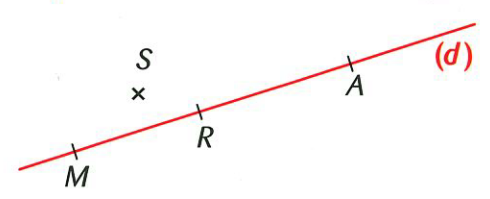
\includegraphics[scale=0.55]{img/droite1}
	\end{center}

	\begin{itemize}
		\item La droite $(d)$ passant par les points $M$ et $R$ se note 
		\item Le point A appartient à la droite $(MR)$, on note :
		\item Le point S n'appartient pas à la droite $(MR)$, on note :
	\end{itemize}
\end{myex}

\begin{mydef}
	Une \kw{\hspace*{5cm}} est une portion de droite limitée d'un seul côté par un point, son \hspace*{5cm}.
\end{mydef}

\begin{myprop}
	La demi-droite d'origine $A$ et passant par $B$ se note 
\end{myprop}

\begin{myex}
	\begin{center}
		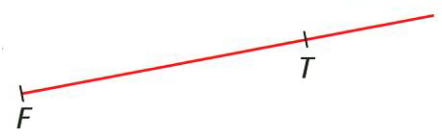
\includegraphics[scale=0.55]{img/demi-droite}
	\end{center}

	La demi droite 
\end{myex}

\begin{mydef}
	Un \hspace*{5cm} est une portion de droite limitée par deux points : ses \hspace*{5cm}.
\end{mydef}


\begin{myprop}
	Le segment d'extrémités $A$ et $B$ se note $\qquad$ ou $\qquad$.
\end{myprop}

\begin{myex}
	\begin{center}
		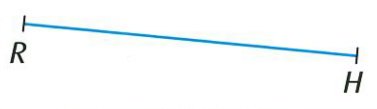
\includegraphics[scale=0.55]{img/segment}
	\end{center}
	
	Le segment 
\end{myex}